% Graphical model for the accelerating accumulator (Fig 1, block A).
% Title-less variant of fig1_graphical_model.tex: the "(A) accelerating
% accumulator" node is dropped so the composite figure's own panel label (A)
% is the only header. Build: pdflatex fig1_gm_notitle.tex; pdftoppm -png -r 300.
\documentclass[border=8pt]{standalone}
\usepackage{tikz}
\usepackage{amsmath}
\usetikzlibrary{positioning,calc,fit,arrows.meta,backgrounds}
\tikzset{
  lat/.style ={circle, draw=black, line width=0.45mm, fill=white,    minimum size=1.25cm, inner sep=1pt, font=\large},
  det/.style ={rectangle, rounded corners=3pt, draw=black, line width=0.45mm, fill=blue!7, minimum height=0.95cm, inner sep=5pt, font=\large},
  obs/.style ={circle, draw=black, line width=0.45mm, fill=black!14,  minimum size=1.25cm, inner sep=1pt, font=\large},
  inp/.style ={circle, draw=black!55, dashed, line width=0.4mm, fill=white, minimum size=0.95cm, inner sep=1pt, font=\normalsize},
  pl/.style  ={draw=black!50, line width=0.35mm, rounded corners=5pt, inner sep=9pt},
  pll/.style ={font=\small\itshape, black!55},
  e/.style   ={-{Latex[length=3mm]}, draw=black!75, line width=0.45mm},
}
\begin{document}
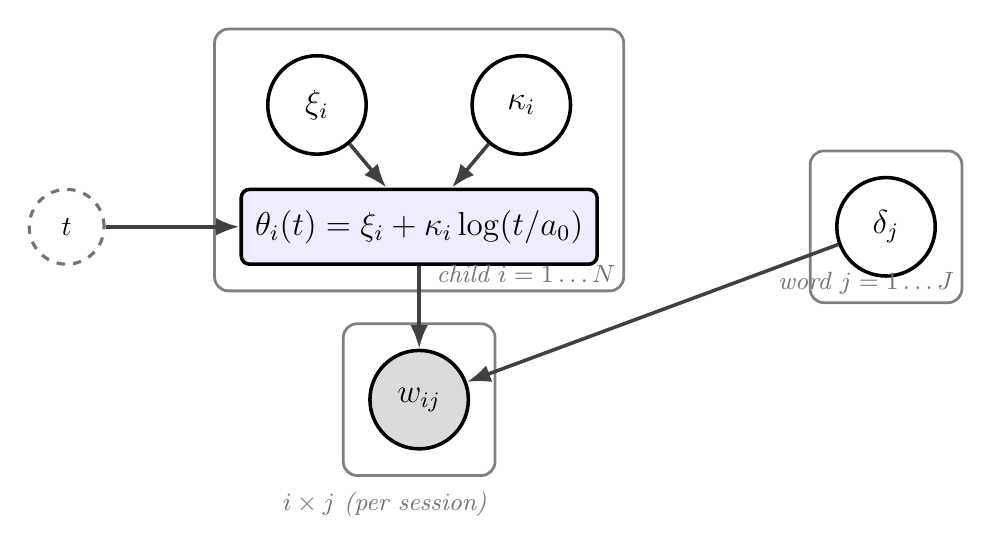
\begin{tikzpicture}[node distance=1.0cm and 1.3cm]
\node[lat] (xi)    {$\xi_i$};
\node[lat, right=of xi] (ka) {$\kappa_i$};
\coordinate (xk) at ($(xi)!0.5!(ka)$);
\node[det, below=1.05cm of xk] (th) {$\theta_i(t)=\xi_i+\kappa_i\log(t/a_0)$};
\node[inp, left=1.7cm of th] (t) {$t$};
\node[obs, below=1.05cm of th] (w) {$w_{ij}$};
\node[lat, right=3.0cm of th] (de) {$\delta_j$};
\draw[e] (xi) -- (th); \draw[e] (ka) -- (th); \draw[e] (t) -- (th);
\draw[e] (th) -- (w);  \draw[e] (de) -- (w);
\begin{scope}[on background layer]
\node[pl, fit=(xi)(ka)(th)] (childpl) {};
\node[pl, fit=(de)] (wordpl) {};
\node[pl, fit=(w)] (obspl) {};
\end{scope}
\node[pll, anchor=south east] at (childpl.south east) {child $i=1\ldots N$};
\node[pll, anchor=south east] at (wordpl.south east) {word $j=1\ldots J$};
\node[pll, anchor=north east] at ([yshift=-2pt]obspl.south east) {$i\times j$ (per session)};
\end{tikzpicture}
\end{document}
